\chapter{Architecture overview}
This chapter can be regarded as a self-contained, high level overview of the implementation details of our system. We start by presenting the main principles we follow in our design. Next, we provide an overview of the system's architecture and the implemented functionality. Lastly, we outline the specification and setup of our honeypot environment.

\section{Principles}
In the implementation of our system, we follow three high-level principles:

\begin{enumerate}
\item We aim to keep each conversation thread going for as long as it is possible. To achieve this, we incorporate various machine learning and natural language processing techniques into the design of our system, and attempt to mimic human performance in the composition of outgoing messages as much as possible.
\item We aim for full system automation. No user interaction should be necessary for the system to function. In order to achieve this, we incorporate a collectors subsystem, classifier and probabilistic finite state models into our design, in order to automatically collect, categorize, and compose messages.
\item We aim to build a safe and secure system. In order to do this, we run our system from a secure remote server and use anonymous email accounts for sending and receiving emails. In addition, we ensure our natural language modules provide only fictitious details in conversations with scammers.
\end{enumerate}

\section{Overview}
The main functionality of the system is split into five major components -- collection, information extraction, classification, identity generation and response generation. These components operate together to obtain AFF emails, perform information extraction and classification tasks, generate and maintain the agent's identity and compose replies. This is illustrated in Figure 3.1.

\begin{figure}[h]
	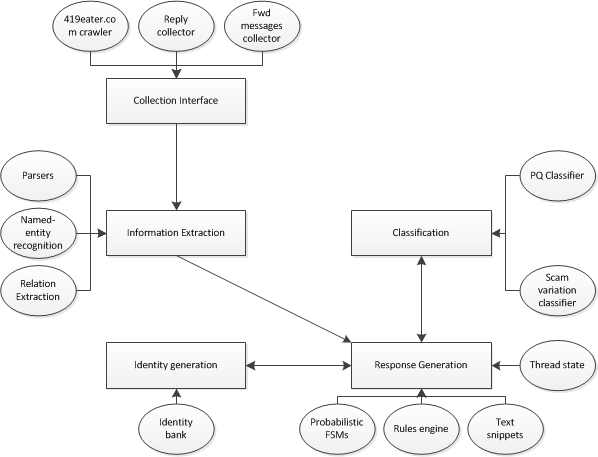
\includegraphics{pics/system_smaller.png}
	\caption{System architecture overview}
\end{figure}


\subsection*{Collection}
The collection component defines an interface for entering new messages into the system. This interface is thread-safe and allows for multiple collector modules to run simultaneously. It is also extensible, so creation of new collector modules is easy. For the purposes of this project, we have implemented three message collectors -- a crawler and scraper for 419eater.com, a reply collector, and forwarded messages collector. The crawler and scraper is designed to download surplus 419 scam letters from the aforementioned web site. The reply collector simply iterates over all email boxes maintained by our agent and downloads any received messages. Finally, the forwarded message collector monitors a mailbox, where people can forward their spam messages and the collector will automatically filter out any personally identifiable information before passing them into the system. These three collectors ensure a constant flow of new messages into the system and automate the process of fetching replies to existing conversation threads. The collection component is explained in more detail in Chapter 4.

\subsection*{Information extraction}
The information extraction component provides a set of algorithms for extracting useful information from incoming messages. As this is the first step of processing after entry into the system, these algorithms are also equipped to deal with potentially dirty data -- e.g. malformed email headers, message body, etc. The main tasks performed by this component are named-entity recognition, email extraction, removing HTML, removing quoted messages, header parsing, relations extraction. Some of these tasks are challenging -- e.g., given a set of emails and named entities, compute named entity, email pairs that refer to the same person. Others appear trivial, but are also difficult -- e.g., it is hard to separate a quoted message from the body of an email message, as there is no universally observed standard on messages should be quoted on reply. We go into further detail on these problems and the proposed solutions in Chapter 5.

\subsection*{Classification}
The classification component provides a wrapper interface to an instance of the Stanford Classifier \cite{P13}. The Stanford package is a Java implementation of a maximum entropy classifier. Maximum entropy models maximize the conditional likelihood of classes and their weights take feature dependence into account, which make them particularly suitable for text classification tasks. For the purposes of this project, we have trained two classifiers. Our first classifier is used to determine which one of the 22 recognized AFF variation is in play for incoming messages and has F$_{1} = 81.177$. The second model, the PQ classifier, is a binary classifier used to determine whether a message contains a request for personal information. As we previously discussed in Section 2.1, this is an opportunity for us to gain the scammer's trust. The PQ classifier has a F$_{1}$ score of 86.667. Feature selection, methodology and results for both classifiers are discussed in detail in Chapter 6.

\subsection*{Identity generation}
The identity generation component is tasked with providing the agent with a personality. In the context of AFF scams, this means a name, age, occupation, email address, postal address, country, marital status. This information is fictitious and may be used by the response generation component, depending on the state of the conversation and the current strategy. An identity is attached to each conversation thread in order to ensure consistency. The component provides the facilities required to obtain and manage identities. It is discussed in more detail in Section 7.1.

\subsection*{Response generation}
The response generation component takes in as inputs the result of the information extraction tasks, an identity, the message, and its class. It then composes a response and sends it to the scammer. This is accomplished in three steps. The first step is to determine whether the incoming message belongs to a thread. We define a thread as a logical unit of all messages related to a single instance of a scam. Because a thread can contain more than two participants, we propose a bucketing algorithm to group messages together. Second, once a thread is selected (or a new thread is created), based on the recorded state of the conversation, message class, PQ classifier, and class-specific rules, a hierarchy of finite state machines generates a response. The response is generated in multiple stages. The first a top-level FSM builds a template, which is then filled out by lower-level probabilistic finite state machines (PFSMs) with snippets of text or recursive calls to another set of PFSMs. In the final step, the component opens a connection to a SMTP server and pushes out the message. Further implementational detail on response generation is provided in Chapter 7.

\section{Honeypot environment}

To satisfy the personal safety requirements of this project, we require a customized setup that does not expose the author's IP address, identity or a link to the University of Edinburgh.

Because of that, we run our prototype system on a leased virtual private server. The virtual machine features 4 GB RAM, Intel Xeon 2.80 GHz CPU, CentOS 6 (Linux kernel 3.0.22) and is secured through a firewall that blocks all incoming traffic, except secure shell access. The physical server is located in a data center in London and is managed by clustered.net. For sending and receiving emails, we use free anonymous email accounts set up on Yahoo! Mail and GMX. Connections to the POP3 and SMTP servers are secured with SSL. The minimum deployment environment requirements for the prototype system are: Python $>=$ 2.7.2, Oracle Java $>=$ 1.6.0, Beautiful Soup, Stanford Classifier $>=$ 2.1.3, Stanford NER $>=$ 1.2.2. 
